\documentclass[12pt,fleqn]{article}
%\documentclass[12pt,a4paper]{article}
\usepackage{amsmath,epsfig,epsf,psfrag,natbib,lineno,hyperref,setspace}
%\usepackage{a4wide,amsmath,epsfig,epsf,psfrag}
\usepackage[nolists,nomarkers]{endfloat}


\begin{document}

\doublespacing

\textbf{Simultaneous modelling of movement, measurement error, and observer dependence in double observer distance sampling surveys}

\linenumbers

\bigskip

\textbf{Abstract}: Wildlife researchers often use detections, non-detections and recorded distances of animals encountered in transect surveys to estimate abundance. However, commonly available distance sampling estimators require that distances to target animals are made without error and that animals are stationary while sampling is being conducted.  In practice these requirements are often violated. In this paper, we describe a marginal likelihood framework for estimating abundance from double observer data that can accommodate movement and measurement error.  In particular, we suppose that two observers independently detect and record binned distances to observed animal groups, and that they record a binary indicator for whether animals were moving or not.  Under this framework, stationary animals are subject to measurement error and moving animals are subject to both movement and measurement error.  Integrating over unknown animal locations, we construct a marginal likelihood for detection, movement, and measurement error parameters. Estimates of animal abundance can then by obtained via a modified Horvitz-Thompson-like estimator.  Unmodelled heterogeneity in detection probability can potentially be incorporated via observer dependence effects.  We investigate the performance of our approach in a simulation study and by analyzing data from a waterfowl helicopter survey.


\textbf{Key words}: aerial survey, mark-recapture distance sampling, measurement error, movement, point independence



\def\VAR{{\rm Var}\,}
\def\COV{{\rm Cov}\,}
\def\Prob{{\rm P}\,}
\def\bfX{\bf X}
\def\bfbeta{\boldsymbol{\beta}}
\def\bfdelta{\boldsymbol{\delta}}
\def\bfeta{\boldsymbol{\eta}}
\def\bfphi{\pmb{\phi}}
\def\bftheta{\pmb{\theta}}
\def\bfpsi{\pmb{\psi}}
\def\bfPsi{\pmb{\Psi}}
\def\bfpi{\pmb{\pi}}
\def\bfp{{\bf p}}
\def\bfGamma{\pmb{\Gamma}}




\section{Introduction}

Distance sampling surveys \citep{BurnhamEtAl1980,BucklandEtAl2001} are often used to estimate the abundance of wildlife populations.  Historically, such surveys were implemented using a single observer who followed a transect line and recorded the perpendicular distance to each detected animal group.  Assuming 100\% detection on the transect line, models can be fitted to these data that estimate abundance over the surveyed area while accounting for detection probabilities that decrease with distance from the transect line.

More recently, investigators discovered that double observer surveys have some large advantages over single observer surveys.  For instance, one can use the detection/non-detection records to relax the assumption of 100\% detection on the transect line \citep{BorchersEtAl1998}, a crucial development for many species and sampling situations (e.g. aerial surveys).  Analysis of double observer distance data is now canonically referred to as ``mark-recapture distance sampling" (MRDS) because there is a detection history (i.e. binary detection/nondetection records for each observer) in addition to recorded distances. Analysis of these histories could potentially be done in a similar manner to a two sample mark-recapture experiment, although this approach ignores some additional information contained in the distribution of observed distances \citep{LaakeBorchers2004}.

Several different observer configurations are possible within an MRDS estimation framework \citep{BurtEtAl2014}.  In an ``independent" configuration, observers search for animals independently.  Under this configuration it is possible to try to account for heterogeneity in detection probabilities (e.g. visual distinctiveness of different animal groups) by modelling lack of fit between the distribution of observed distances and estimated detection probabilities as a function of distance \citep{LaakeBorchers2004,BorchersEtAl2006,BucklandEtAl2010}.   Alternatively, in a ``trial" configuration \citep{LaakeBorchers2004}, one observer searches ahead, while another searches closer to the survey platform.  Under this configuration, detections by the first observer are used as trials for the second observer.  Collecting data in this manner can be useful for reducing the biasing influence of responsive movement of animals, but at the cost of no longer being able to model heterogeneity in detection probability \citep{BurtEtAl2014}.

In this paper, we develop an integrated likelihood framework to account for movement and measurement error within an independent observer MRDS framework.  Our objective is to account for the biasing effects of measurement error and responsive movement while also being able to model individual heterogeneity through an observer dependence specification.  The effect of movement on distance sampling estimators has previously been examined by \citet{GlennieEtAl2015}, who showed movement could cause considerable bias in distance-based abundance estimators.  However, we have not found any papers that attempt to explicitly model movement.  By contrast, a number of authors have proposed models that account for measurement error in specific distance sampling applications \citep[see e.g.][and references therein]{BorchersEtAl2010}.

The remainder of this article is structured as follows.  First, we describe a motivating data set, in which distance, detection histories, and individual covariates are assembled from a double observer waterfowl aerial survey.  Second, we describe a maximum marginal likelihood framework for analyzing these data.  Under our framework, locations of an animal group seen by the first observer and the second observer are treated as two latent variables.  Next, we illustrate application of our approach by conducting a simulation study and applying it to the waterfowl data set.  We conclude with a short discussion.


\section{Waterfowl data}

In June of 2014, biologists conducted a pilot double observer helicopter survey of Arctic bird species in the Queen Maud Gulf Migratory Bird Sanctuary (Nunavut, Canada). The birds surveyed were predominantly waterfowl, but also included cranes and ptarmigan; we refer to them collectively as waterfowl for the remainder of the paper. The purpose of this particular survey was not to estimate abundance over the whole area. Rather, researchers were interested in comparing estimates of detection probability from double observer survey methods to estimates of detection probability using single observer protocols.
The survey is described in greater detail elsewhere \citep{AlisauskasConn2017}, but we briefly provide information relevant to the analysis provided in this paper.

In the survey, two observers on the same side of the helicopter independently detected and recorded the perpendicular distance from the transect line to each bird group they observed.  Distances were binned into 6 classes: 0-40m, 40-80m, 80-120m, 120-160m, 160-200m, and 200m+.  They also recorded species, the number of waterfowl in each detected group (``group"), and a binary indicator for whether the waterfowl group was flapping their wings (``moving").  These data were previously analyzed by \citet{AlisauskasConn2017}, who used standard MRDS methods that ignored movement and measurement error in their analysis.  Their analysis suggested higher detection probabilities for moving individuals, larger group sizes, and for the front seat observer (relative to a rear seat observer).  They also estimated similar species effects on detection for 7 of the 9 species analyzed; here, we pool data from these 7 species to form an illustrative dataset.  This protocol led to a total of 1025 unique waterfowl group detections; 323 were detected by both observers, 353 by the front observer only, and 258 by the back observer only.  Note that the the back observer's view of the first distance bin was partially obstructed.  A plot of observed distance deviations suggests responsive movement away from the aircraft for moving animal groups.  There were also some minor distance discrepancies for animal groups that were not moving, which is suggestive of measurement error (Fig. \ref{fig:dist_hists}).  Our objective is to build models that formally account for movement and measurement error processes.

\section{Model development}


Consider a double observer MRDS survey where observers independently record binned distances to detected groups of animals and a total of $n$ animal groups are encountered by at least one observer (see Table \ref{tab:notation} for a complete list of notation).  We develop a two stage approach for estimating abundance in the surveyed area from such data.  In the first step, a marginal likelihood framework is used to simultaneously estimate parameters of detection, movement, and measurement error processes.  In the second, a Horvitz-Thompson-like estimator is used to estimate abundance conditioned on parameter estimates from step 1 (a bootstrap procedure is used to quantify precision).  For purposes of this paper we do not explicitly consider the problem of extrapolating abundance/density to a larger region (e.g. to unsurveyed locations); we touch on this issue in the Discussion.

In MRDS surveys with binned distances, observers record animals as occurring in one of $n_\mathcal{S}$ perpendicular distance bins, $\mathcal{S} = \mathcal{S}_1,\mathcal{S}_2,\hdots,\mathcal{S}_{n_\mathcal{S}}$.  Detection probability typically decreases with distance from the transect line, and the maximum distance bin is often set such that animals further away are poorly detected and can be ignored without greatly affecting precision of abundance estimates.  Movement and measurement error introduce complications: animals can potentially move into or out of $\mathcal{S}$, and animals outside of $\mathcal{S}$ can be detected in $\mathcal{S}$.  For these reasons, the models we develop rely on augmenting $\mathcal{S}$ with additional distance bins to allow for movement and measurement error (Fig. \ref{fig:aug_bins}).  Call this augmented set $\mathcal{Z}$.

Let $y_{oi}$ be a binary indicator for whether or not the $i$th animal group was detected by observer $o$.  Similarly, let $d_{oi}$ denote the distance bin recorded by observer $o$ for animal group $i$ (note $d_{oi}$ is only defined when $y_{oi}=1$). Letting bold lower case symbols denote vectors (e.g. ${\bf y}_{o \cdot}$ gives a sequence of detections for observer $o$, $i=1,2,\hdots,n$) and bold upper case symbols denote matrices, we seek to define a marginal likelihood $[\boldsymbol{\theta} | {\bf Y},{\bf D}, {\bf X}]$, where $\boldsymbol{\theta}= \{ \boldsymbol{\beta,\phi,\varphi} \}$ are parameters describing detection, movement, and measurement error, and ${\bf X}$ include individual covariates collected for each animal group that can be used to explain variation in detection probabilities.

\subsection{Likelihood}

To construct such a likelihood, we start with the general framework proposed by \citet{BorchersEtAl2015} for spatial mark-recapture and distance sampling surveys.  Conditioning on detection, Borchers et al. suggested that the joint distribution of animal locations and detections could be written as a product of (1) a joint probability density function for the latent locations of animals, and (2) a joint probability mass function for the encounter histories conditional on location.  We expand upon this framework to allow movement to affect the distribution of animal locations and to incorporate a measurement error mechanism.

Letting ${\bf z}_o$ denote the true locations of animals when they enter the field of view of observer $o$, we write the joint probability mass function of observed data as a product of
\begin{enumerate}
   \item $[{\bf Z}|\boldsymbol{\theta}]$, a bivariate probability mass function for the distribution of true animal locations, given detection by at least one observer; and
   \item $[{\bf Y},{\bf D}|{\bf Z},\boldsymbol{\theta},{\bf X}]$, a model for binary detections and observed distances given true unobserved locations and individual detection covariates; and
\end{enumerate}
If we knew the true locations of observed animals, we could simply base inference on the likelihood
\begin{eqnarray*}
  [\boldsymbol{\theta} | {\bf Y},{\bf D}, {\bf X}] & \propto & [{\bf Z}|\boldsymbol{\theta}][{\bf Y},{\bf D}|{\bf Z},\boldsymbol{\theta},{\bf X}].
\end{eqnarray*}
However, we do not know the actual animal locations so instead integrate (sum) over an augmented set of distance bins $\mathcal{Z}$ that could plausibly have resulted in a detection (see \textit{Distribution of animal locations} for more discussion of bin augmentation).
As such, we write the joint marginal likelihood of detection, movement, and measurement error parameters as
\begin{eqnarray}
  [\boldsymbol{\theta} | {\bf Y},{\bf D}, {\bf X}] & \propto & \prod_i \left( \sum_{z_{i1} \in \mathcal{Z}} \sum_{z_{i2} \in \mathcal{Z}} [{\bf z}_{i \cdot} |\boldsymbol{\theta}][{\bf y}_{i \cdot},{\bf d}_{i \cdot}|{\bf z}_{i \cdot} , \boldsymbol{\theta} , {\bf x}_i]
   \right).
  \label{eq:lik}
\end{eqnarray}
We now describe each of the likelihood components in further detail.

\subsubsection{Distribution of animal locations}

The first component of the likelihood (Eq. \ref{eq:lik}) is the joint probability mass function for the locations of group $i$, $[{\bf z}_{i \cdot} |\boldsymbol{\theta}]$ given detection by at least one observer.  We write this distribution as a function of (i) an initial state distribution, (ii) a movement kernel, and (iii) a thinning probability equivalent to detection probability by at least one observer.  Specifically, we set
\begin{eqnarray}
[{\bf z}_{i \cdot} |\boldsymbol{\theta}] & \propto & [z_{i1}][z_{i2}|z_{i1},\boldsymbol{\phi}]p_i^*(z_{i1},z_{i2}|{\bf x}_i,\boldsymbol{\beta},\boldsymbol{\phi},\boldsymbol{\varphi}).
\end{eqnarray}
In all applications described in this paper, we make the assumption that the first observer (typically in a front seat) detects animal groups before any responsive movement has occurred.  Under this assumption, random placement of transect lines should help ensure that perpendicular distances of animals from the transect line are uniformly distributed in space \citep[cf.][]{BucklandEtAl2001}.  Letting $\pi_j$ denote the proportional diameter of distance bin $j$ (i.e. $\pi_j = a_j / \sum_k a_k$ where $a_j$ is the diameter of of distance bin $j$), we simply have
\begin{eqnarray*}
  [z_{i1}] & = & \text{Categorical}(\pi_1,\pi_2,\hdots,\pi_{n_{\mathcal{Z}}}),
\end{eqnarray*}
where it is understood that ``Categorical" denotes a multinomial distribution with index 1, and $n_{\mathcal{Z}}$ is the number of latent distance bins.

Next, the bivariate movement pmf $[z_{i2}|z_{i1},\boldsymbol{\phi}]$ describes the location of animal group $i$ when it enters the field of view of observer 2 as a function of the location when it was in the field of view of observer 1.  We model this as another categorical distribution:
\begin{eqnarray*}
  [z_{i2}|z_{i1},\boldsymbol{\phi}] & = & \text{Categorical} \left( \psi(z_{i1},1),\psi(z_{i1},2),\hdots,\psi(z_{i1},n_\mathcal{Z}) \right).
\end{eqnarray*}
For applications in this paper, we parameterize the movement transition kernel probabilities $\boldsymbol{\psi}$ using asymmetric kernels.  Using an asymmetric kernel can allow movement rates to be different toward and away from the transect line (anticipating a behavioral response to the survey platform). In particular, we set
\begin{linenomath*}
\begin{equation}
  \psi(z_{i1},z_{i2}) \propto g(z_{i1},z_{i2}|\boldsymbol{\phi}) \text{, where}
  \label{eq:psi}
\end{equation}
\begin{equation}
  g(z_{i1},z_{i2}) = \left\{ \begin{array}{rl}
                                    f(\delta_{i2}|\mu=\delta_{i1},\sigma=\phi_1) & z_{i2}<z_{i1}, m_i = 1 \\
                                    f(\delta_{i2}|\mu=\delta_{i1},\sigma=\phi_2) & z_{i2} \ge z_{i1}, m_i = 1  \\
                                    1.0 & z_{i2}=z_{i1}, m_i=0 \\
                                    0.0 & z_{i2} \ne z_{i1}, m_i=0
                                    \end{array} \right.
  \label{eq:g}
\end{equation}
\end{linenomath*}
Here, $f()$ gives a probability density function; in our examples, we consider Laplace (double exponential) and Gaussian distributions as choices for $f()$. Note that $\delta_{io}$ gives the perpendicular distance from the transect line to the midpoint of distance bin $z_{io}$.  Also note that we assume that stationary animals (i.e. with $m_i=0$) do not change distance bins.

Finally, the thinning probability
$p_i^*(z_{i1},z_{i2}|{\bf x}_i,\boldsymbol{\beta},\boldsymbol{\phi},\boldsymbol{\varphi})$ describes the probability of being detected by at least one observer for an animal that is in distance bin $z_{i1}$ at time 1 and $z_{i2}$ at time 2. For generality, we calculate probability as the sum of obtaining one of the three possible detection histories: 11, 10, or 01 (detected by both observers, detected by the front observer but not the back, or detected by the back observer but not the front).  In particular,
\begin{eqnarray*}
  p_i^*(z_{i1},z_{i2}|{\bf x}_i,\boldsymbol{\beta},\boldsymbol{\phi},\boldsymbol{\varphi}) & = &
  p_{i1}(z_{i1}) \omega(z_{i1},\mathcal{S}) p_{i2}(z_{i2})
  \omega(z_{i2},\mathcal{S}) + \\
   & & p_{i1}(z_{i1})\omega(z_{i1},\mathcal{S}) \left[
   p_{i2}(z_{i2})(1-\omega(z_{i2},\mathcal{S}))+(1-p_{i2}(z_{i2})) \right] + \\
   & & p_{i2}(z_{i2})\omega(z_{i2},\mathcal{S}) \left[
   p_{i1}(z_{i1})(1-\omega(z_{i1},\mathcal{S}))+(1-p_{i1}(z_{i1})) \right].
\end{eqnarray*}
This expression is slightly different than typically encountered in mark-recapture calculus, as one must account for two ways of getting a 0 in a capture history: an observer can miss the animal group, or an observer can detect the group but determine it is out of the truncation range of the transect (i.e. $\notin \mathcal{S}$).  To account for the latter possibility, we make use of the measurement error kernel $\boldsymbol{\omega}$ (Table \ref{tab:notation}), which can be parameterized similarly to $\boldsymbol{\phi}$ (see Eqs. \ref{eq:psi}-\ref{eq:g}).  In applications in the paper, we consider use of symmetric kernels (Gaussian or Laplace) with a single dispersion parameter, $\varphi$.  Our expression for $p_i^*$ also relies on individual- and observer-dependent detection probabilities, $p_{io}(z_{io})$.  In order to impart meaningful variation in detection probability, it is useful to express these in a regression framework on a logit-linear scale, such that
\begin{eqnarray}
  \textrm{logit}({\bf p}) & = & {\bf X} \boldsymbol{\beta}.
\end{eqnarray}
Note that we write $p_{io}$ as a function of $z_{io}$ to emphasize that the design matrix ${\bf X}$ will often depend on the latent position of animals.

\subsubsection{Likelihood of observed detections}

The next component of the the likelihood is $[{\bf y}_{i \cdot},{\bf d}_{i \cdot}|{\bf z}_{i \cdot} , \boldsymbol{\theta} , {\bf x}_i]$, the probability of observing the particular detection history and distance bin values for animal group $i$ conditional on animal location.  Conditional on detection by at least one observer, there are again three possible types of encounter histories: $11$, $10$, or $01$.  For $11$ histories, there are $n_\mathcal{S}^2$ combinations of possible recorded distance bins; for $10$ histories, there are $n_\mathcal{S}$ distance bins possible for observer 1; for $01$ histories, there are $n_\mathcal{S}$ distance bins possible for observer 2.  Thus, we can view $[{\bf y}_{i \cdot},{\bf d}_{i \cdot}|{\bf z}_{i \cdot} , \boldsymbol{\theta} , {\bf x}_i]$ as a multinomial distribution with index 1 and $n_\mathcal{S}^2 + 2 n_\mathcal{S}$ possible outcomes. The likelihood contribution for a particular animal group $i$ can thus be written as
\begin{equation*}
    p_i^* \times  \left\{ \begin{array}{rl}
    p_{i1}(z_{i1}) \omega(z_{i1},d_{i1}) p_{i2}(z_{i2}) \omega(z_{i2},d_{i2}) & \text{if }y_{i1}=y_{i2}=1 \\
    p_{i1}(z_{i1})\omega(z_{i1},d_{i1}) \left[
    p_{i2}(z_{i2})(1-\omega(z_{i2},\mathcal{S}))+(1-p_{i2}(z_{i2})) \right] &  \text{if } y_{i1}=1, y_{i2}=0 \\
    p_{i2}(z_{i2})\omega(z_{i2},d_{i2}) \left[
    p_{i1}(z_{i1})(1-\omega(z_{i1},\mathcal{S}))+(1-p_{i1}(z_{i1})) \right]
                                     &  \text{if } y_{i1}=0, y_{i2}=1.
                                    \end{array} \right.
\end{equation*}





\subsection{Horvitz-Thompson-like abundance estimator}

\subsection{Extension to incorporate detection heterogeneity}


\section{Analysis of waterfowl data}

\section{Simulation studies}

\section{Discussion}

extrapolation to unsurveyed areas.

additive vs. multiplicative measurement error \citep{BorchersEtAl2010}

influence of proportion moving (assumed 0.7 in sim study).

other errors (group size differences, flying/not flying, species, etc.)

\section{Data accessibility}
R scripts and data necessary to recreate analyses have been collated into an R package, which is currently available at \url{https://github.com/pconn/MSmixture}.  We plan to publish the package to an online archive/repository upon acceptance. \\


\bibliographystyle{ECA_jasa}
\bibliography{master_bib}


\pagebreak
\begin{table}[ht]
\caption{Definitions of fixed and estimated quantities for the MRDS model incorporating movement and measurement error.
}
\label{tab:notation}
\raggedright
\begin{tabular}{p{2cm}p{13cm}}
  \hline
   Quantity & Definition \\
  \hline
   \multicolumn{2}{l}{\textbf{A. Fixed quantities}}   \\
  $n$ & Number of animals detected by at least one observer \\
  $y_{io}$ & Binary indicator for whether animal group $i$ was detected by observer $o$\\
  $d_{io}$ & Distance bin recorded by observer $o$ for animal group $i$ (if recorded) \\
  $m_{i}$ & A binary indicator for whether animal group $i$ was moving when observed (a single determination is made) \\
  ${\bf x}_i$ & A vector of covariates used to explain variation in detection probability for group $i$ \\
  $g_i$ & Number of animals in group $i$ (a single determination is made) \\
  $\mathcal{S}$ & The set of distance bins for which data are recorded, $\mathcal{S}=\mathcal{S}_1,\mathcal{S}_2,\hdots,\mathcal{S}_{n_\mathcal{S}}$ \\
  $\mathcal{Z}$ & The set of latent distance bins used for modeling true animal locations, $\mathcal{Z}=\mathcal{Z}_1,\mathcal{Z}_2,\hdots,\mathcal{Z}_{n_\mathcal{Z}}$
  \\
  $\pi_j$ & Proportion of $\mathcal{Z}$ covered by latent distance bin $j$ \\
  \multicolumn{2}{l}{\textbf{B. Parameters and functions of parameters}} \\
  $z_{io}$ & True (latent) distance bin of group $i$ when encountered by observer $o$ \\
  $\delta_{io}$ & Perpendicular distance from the transect line to the midpoint of bin $z_{io}$ \\
  $\boldsymbol{\beta}$ & A vector of parameters governing logit-linear variation in detection probability \\
  %$\boldsymbol{\beta}_\lambda$ & A vector of parameters governing observer %dependence \\
  $\boldsymbol{\phi}$ & Parameters governing animal movement \\
  $\boldsymbol{\varphi}$ & Parameters governing distance measurement error \\
  $p_{io}(z_{io})$ & Probability that observer $o$ detects group $i$ given that the group is truly in distance bin $z_{io}$\\
  $p_i^*(z_{i1},z{i2})$ & Probability that at least one observer detects group $i$ given the group is in distance bin $z_{i1}$ at time 1 and $z_{i1}$ at time 2\\
  $\psi(z_{i1},z_{i2})$ & Probability that an animal that is in latent distance bin $z_{i1}$ when it passes observer 1 will be in latent distance bin $z_{i2}$ when it passes observer 2 \\
  $\omega(z,d)$ & Probability that an animal group in distance bin $z$ is recorded as being in distance bin $d$ \\
  $\omega(z,\mathcal{S})$ & Probability that an animal group in distance bin $z$ will have a recorded distance bin falling within $\mathcal{S}$ \\
  ${\bf X}$ & A design matrix used to impart logit-linear structure on detection probabilities; note this will often include latent distance values, ${\bf z}_{i \cdot}$  \\
  $N$ & True abundance of animals in the surveyed area \\
\hline
\end{tabular}
\\
%$\dag$ Refitted model; see \textit{Results}.
\end{table}


%\pagebreak
%\begin{table}[ht]
%\caption{A summary of model selection results and estimated abundance for the four models fitted to bearded seal counts.  The models include formulations with or without predictive covariates ($cov=1$ or 0, respectively) , and with or without the preferential sampling parameter $b$ estimated ($b=1$ or 0, respectively) .  All models included spatially autocorrelated random effects on log-scale abundance intensity.  Shown are the log integrated likelihood, the number of fixed effect parameters, $\Delta \textrm{AIC}$, AIC model weights, and estimated apparent abundance over the landscape ($\hat{N}$) together with a Hessian-based standard error estimate.
%}
%\label{tab:aic}
%\raggedright
%\begin{tabular}{lccccc}
%  \hline
%  Model & Log likelihood & Params & $\Delta \textrm{AIC}$ & Wgt & $\hat{N}$(SE) \\
%  \hline
%  $M_{cov=0,b=0}$ & -2667.1 & 3 & 21.7 & 0.00 & 68556 (7408)\\
%  $M_{cov=0,b=1}$ & -2665.3 & 4 & 20.1 & 0.00 & 45857 (5114) \\
%  $M_{cov=1,b=0}$ & -2650.3 & 9 &  0.0 & 0.53 & 59312$^\dag$ (5231)  \\
%  $M_{cov=1,b=1}$ & -2649.4 & 10 & 0.3 & 0.47 & 49826 (10369) \\
%\hline
%\end{tabular}
%\\
%$\dag$ Refitted model; see \textit{Results}.
%\end{table}



\begin{figure*}
\begin{center}
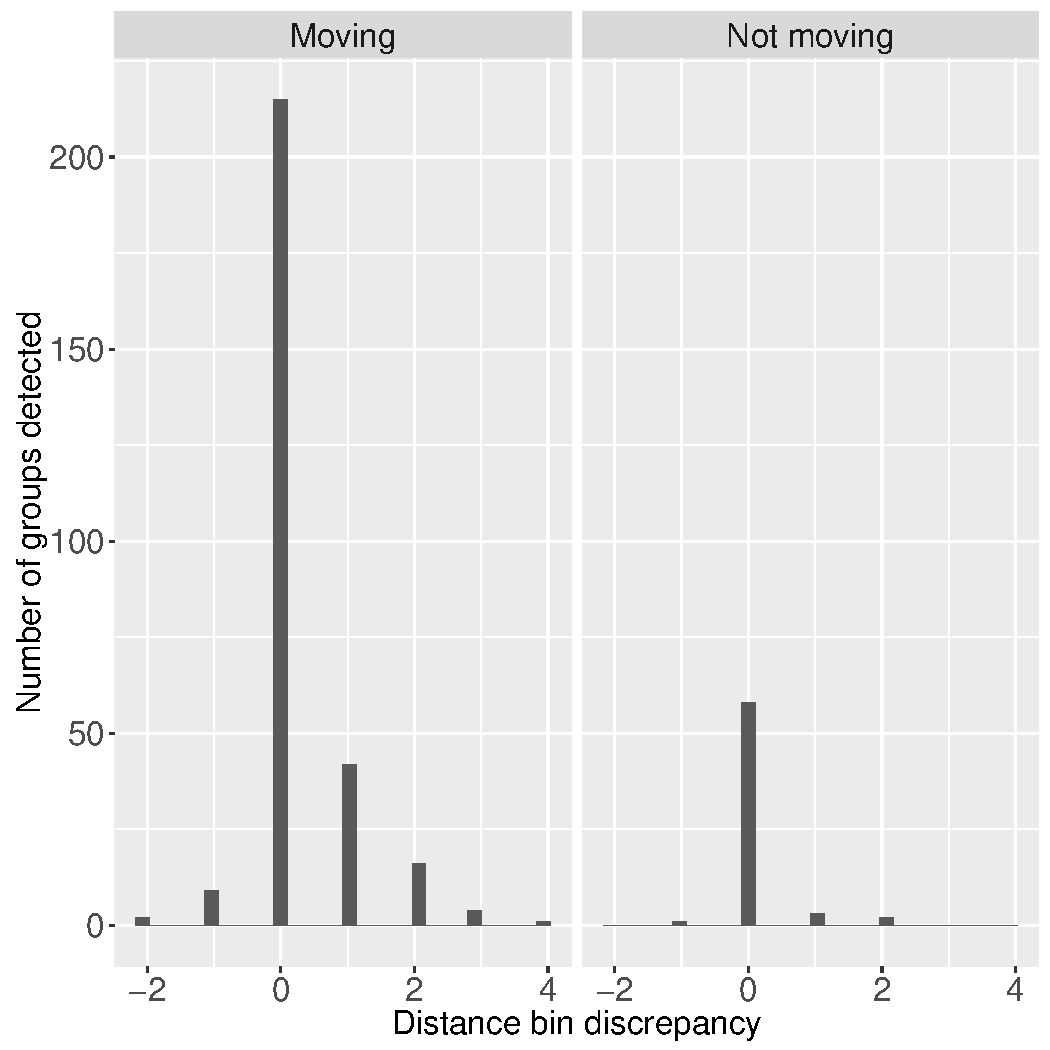
\includegraphics[width=150mm]{Dist_error_hists_JABES.pdf}
\caption{Distribution of distance bin discrepancies ($d_2 - d_1$) for bird groups encountered by both front and back seat observers in aerial surveys.  For moving birds, the distance bin observed by the back observer tended to be further away than the bin observed by the front observer.  Since the second observer invariably detected birds later than the front observer, this suggests responsive movement away from the aircraft. }
\label{fig:dist_hists}
\end{center}
\end{figure*}

\pagebreak
\begin{figure*}
\begin{center}
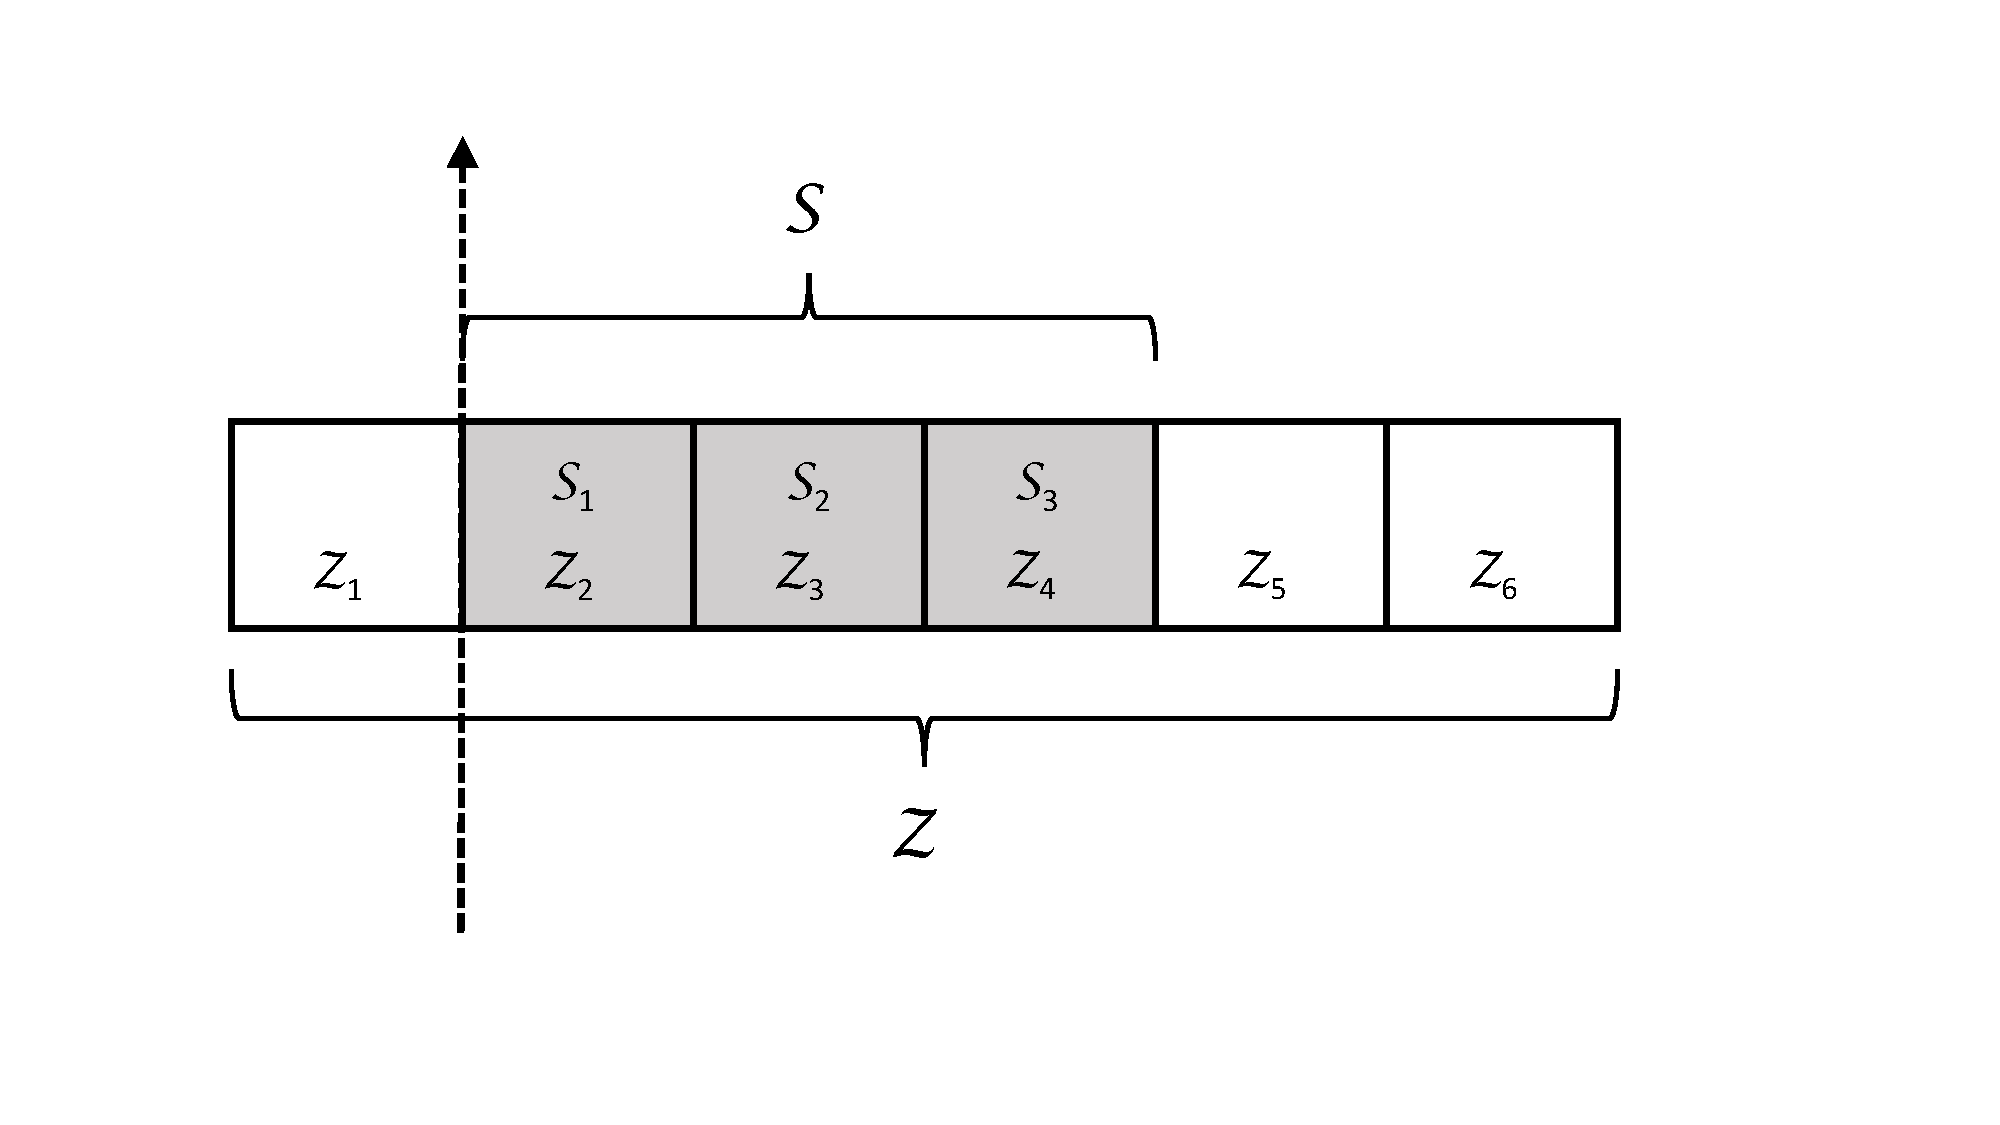
\includegraphics[width=150mm]{augmented_bin_figure.pdf}
\caption{A depiction of observed ($\mathcal{S}$) and latent ($\mathcal{Z}$) distance bins that could potentially be used in analysis of a hypothetical mark-recapture distance sampling (MRDS) survey.  In this example, only animals encountered in one of the three shaded distance bins to the right of the transect line (dashed line) are recorded; however, the state space is augmented with an additional three bins to account for possible animal movement and measurement error.  In practice, the number of augmented distance bins that are needed will be a function of the magnitude of the movement and measurement error processes.}
\label{fig:aug_bins}
\end{center}
\end{figure*}



\end{document}
